\documentclass{article}

% Language setting
% Replace `english' with e.g. `spanish' to change the document language
\usepackage[english]{babel}

% Set page size and margins
% Replace `letterpaper' with `a4paper' for UK/EU standard size
\usepackage[a4paper,top=2cm,bottom=2cm,left=3cm,right=3cm,marginparwidth=1.75cm]{geometry}

% Useful packages
\usepackage{amsmath}
\usepackage{graphicx}
\usepackage[colorlinks=true, allcolors=blue]{hyperref}
\usepackage{xcolor}
\usepackage{listings}
\usepackage{multicol}
\colorlet{mygray}{black!30}
\colorlet{mygreen}{green!60!blue}
\colorlet{mymauve}{red!60!blue}



\lstdefinelanguage{makefile}{
otherkeywords={.SUFFIXES},
morekeywords={SUFFIX, CPP_,},
moredelim=[is][\color{mbleu}]{/*}{*/},
style=global,%
morecomment=[l][commentstyle]{\#},%
emphstyle={\color{vimvert}},%
moredelim=[s][\color{vimvert}]{\$(}{)}%
}

\lstdefinelanguage{cpp}{
  backgroundcolor=\color{gray!10},  
  basicstyle=\ttfamily,
  columns=fullflexible,
  breakatwhitespace=false,      
  breaklines=true,                
  captionpos=b,                    
  commentstyle=\color{mygreen}, 
  extendedchars=true,              
  frame=single,                   
  keepspaces=true,             
  keywordstyle=\color{blue},      
  language=c++,                 
  numbers=none,                
  numbersep=5pt,                   
  numberstyle=\tiny\color{blue}, 
  rulecolor=\color{mygray},        
  showspaces=false,
  showstringspaces=false,
  showtabs=false,                 
  stepnumber=5,                  
  stringstyle=\color{mymauve},    
  tabsize=3,                                     
  title=\lstname 
}
\lstset{language=cpp}
\lstnewenvironment{code}[2][]{%
  \lstset{%
    numbers = left,
    title   = #2,
    #1,
  }%
}{}

\title{Embedded Systems Programming \\ Assignment 5.2 \\ \large Communication between Raspberyr Pi and Arduino}
\author{Steinarr Hrafn Höskuldsson}

\usepackage{fancyhdr}
\fancypagestyle{firststyle}
{
   \fancyhf{}
   \fancyhead[L]{Embedded Systems Programming}
   
   \renewcommand{\headrulewidth}{0pt} % removes horizontal header line
}

\newcommand{\mycomment}[1]{}
\begin{document}
\pagestyle{firststyle}
{\let\newpage\relax\maketitle}

\mycomment{
\begin{figure}[h]
    \centering
    \includegraphics[width=0.75\textwidth]{LAB3/Basic1.png}
    \caption{"Switch test" Breadboard set up}
    \label{fig:Switch_test}
\end{figure}

\lstinputlisting[caption=main.cpp in Part 3]{Assignment3_1StateBehaviour/src/main_prt3.cpp}

}


\section*{Part 1}
The Arduino's tx pin was connected to the Raspberry Pi's rx pin and the Raspberry Pi's tx to the Arduino's rx pin. A logic level converter was used to convert between the 3.3V and 5V logic levels.

\begin{figure}[h]
    \centering
    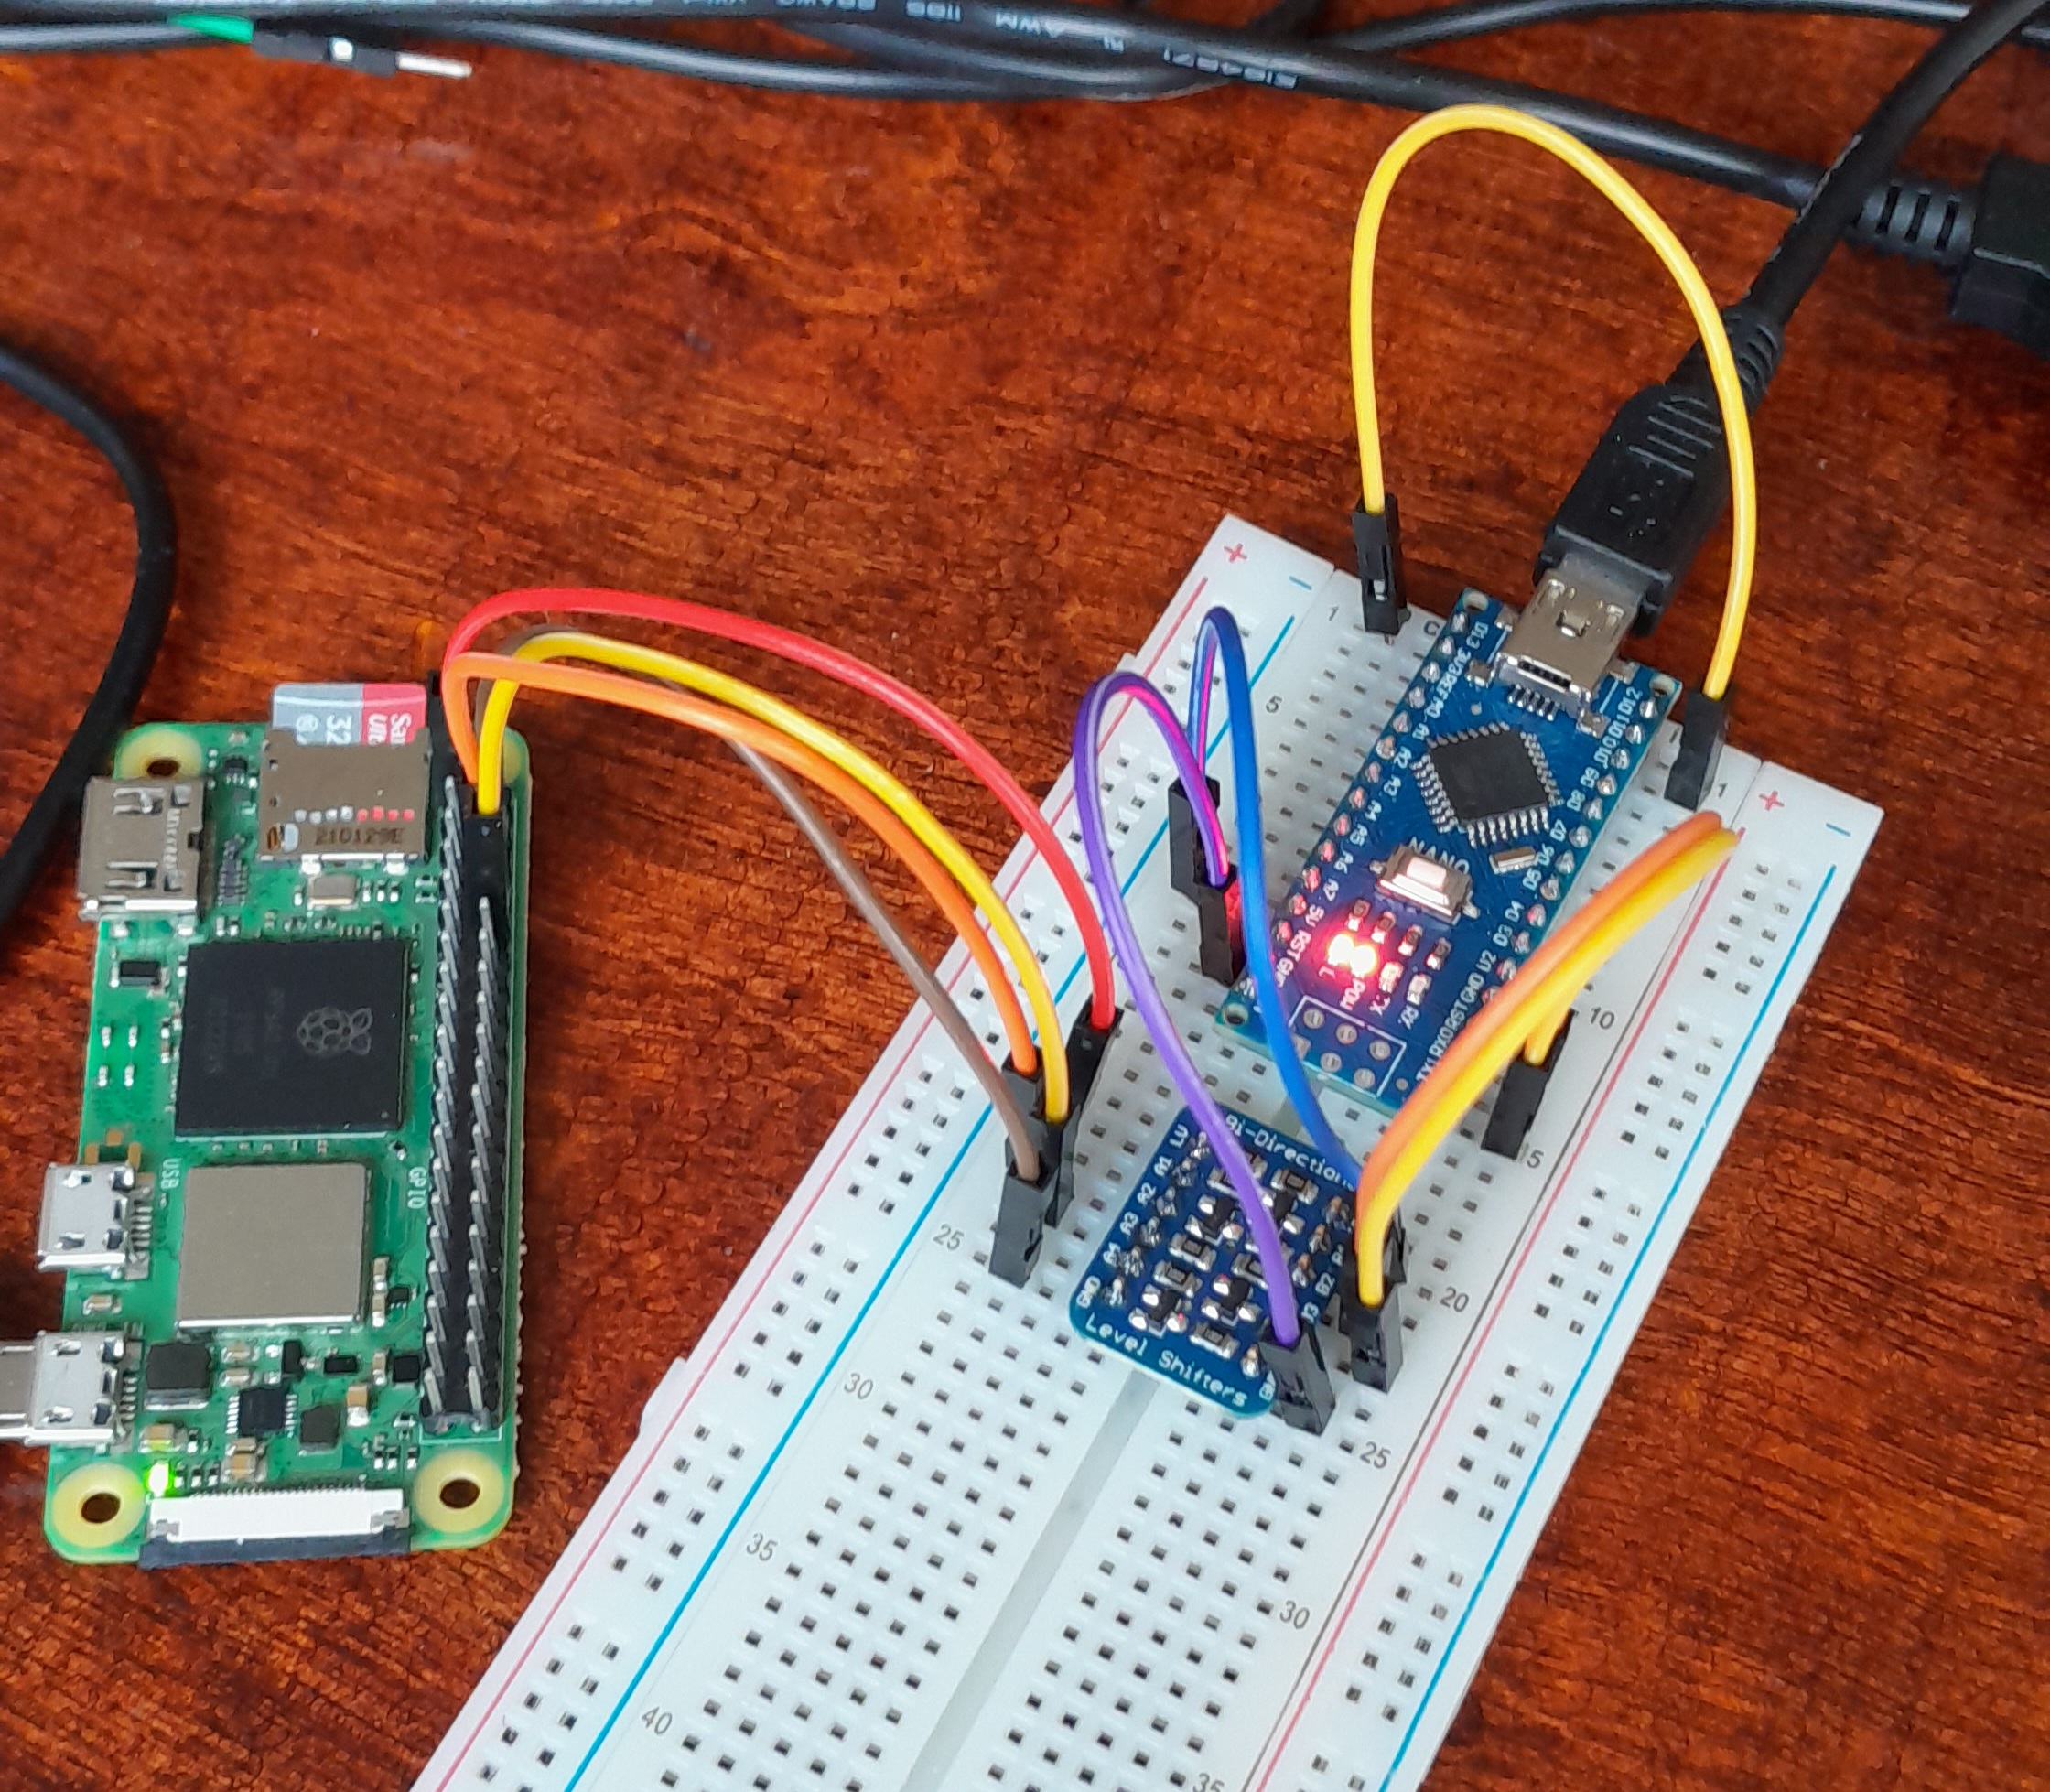
\includegraphics[width=0.75\textwidth]{Assignment5_2Communication/20221025_134104.jpg}
    \caption{A picture of connections between Arduino and Raspberry Pi}
    \label{fig:part1}
\end{figure}

\section*{Part 2}
The supplied Arduino Sketch was uploaded to the Arduino and the supplied command.c program was saved on the Raspberry Pi, compiled with gcc and executed using for example: \verb!./command "LED 100"!. 

The result was that the brightness of the LED could be controlled from the terminal of the Raspberry Pi. The results, as reported by the Arduino, were also printed to the terminal.

The Arduino sketch was then modified to comply with line reading mode by using \verb!Serial.println! instead of \verb!Serial.print! to print the buffer. This resulted in minimal change on the Raspberry Pi side, two new lines were printed in the terminal output and the length of the received string increased by two.

\section*{Part 3}
The Arduino sketch was modified to accept a two byte binary message containing a register byte and a value byte. If the register byte was 2 then the Arduino will write the value byte out as a pwm signal on pin 11.

A new c program was written for the Raspberry Pi that sets the serial port to raw mode and prints the two input arguments as binary values.


\lstinputlisting[caption=Modified Arduino sketch ]{Assignment5_2Communication/arduino_part3.ino}

\lstinputlisting[caption=Modified c program ]{Assignment5_2Communication/src/binmand.c}



\end{document}

